\documentclass[]{article} % A4 paper and 11pt font size

\usepackage{listings} % Required for inserting code snippets
\usepackage[usenames,dvipsnames]{color} % Required for specifying custom colors and referring 

\usepackage[utf8]{inputenc} % Use 8-bit encoding that has 256 glyphs
\usepackage[finnish]{babel} % language/hyphenation
\usepackage{amsmath,amsfonts,amsthm,mathtools} % Math packages
\usepackage{graphicx}
\usepackage{setspace}
\usepackage[margin=1.0in]{geometry}
%\newcommand{\sinc}{\text{sinc}}


\newcommand{\sinc}{\text{sinc}}

\setlength\parindent{0pt}
\setlength{\parskip}{2mm plus1mm minus1mm}



\usepackage{sectsty} % Allows customizing section commands
%\allsectionsfont{\normalfont\scshape} % Make all sections centered, the default font and small caps

\usepackage{fancyhdr} % Custom headers and footers
%\renewcommand{\familydefault}{\sfdefault}

\pagestyle{fancyplain} % Makes all pages in the document conform to the custom headers and footers
\fancyhead{} % No page header - if you want one, create it in the same way as the footers below
\fancyfoot[L]{AVR ja ARM harjorustyö 2015} % Empty left footer
\fancyfoot[C]{} % Empty center footer
\fancyfoot[R]{\thepage} % Page numbering for right footer
\renewcommand{\headrulewidth}{0pt} % Remove header underlines
\renewcommand{\footrulewidth}{0pt} % Remove footer underlines
\setlength{\headheight}{13.6pt} % Customize the height of the header
\numberwithin{equation}{section}
\numberwithin{figure}{section}
\numberwithin{table}{section}

%\usepackage[margin=1.5in]{geometry}
%\addtolength{\topmargin}{-.875in}
%\addtolength{\textheight}{1.75in}
%\setlength\parindent{0pt} % Removes all indentation from paragraphs - comment this line for an assignment with lots of text
% \tolerance=1200


\newcommand{\horrule}[1]{\rule{\linewidth}{#1}} % Create horizontal rule command with 1 argument of height

\title{	
\normalfont \normalsize 
\textsc{Turun ammattikorkeakoulu} \\ [25pt] % Your university, school and/or department name(s)
\huge AVR ja ARM harjorustyö, Ohjelmoinnin jatkokurssi\\ % The assignment title
}
\author{
Jarmo Kivekäs
}
\date{\normalsize\today} % Today's date or a custom date



\begin{document}
\maketitle
\tableofcontents

\newpage












\section{Johdanto}
\label{sec:Johdanto}


Tämä raportti käsittelee robottia joka toteutettiin harjoitustyönä Ohjelmoinnin perusteet kurssia varten.
Harjoitustyön tarkoituksen oli oppia järjestelmäläheistä ohjelmointia ARM sekä AVR ympäristäissä.
Raportin sekä siinä esitetyn materiaalin on laatinut Jarmo Kivekäs.

Monet (jopa suurin osa) työssä toteutetuista asioista olisi voinut toteuttaa yksinkertaisemmin käyttämällä valmiita kirjastoja. Oppimistavoitteiden saavuttamiseksi on keskitytty järjestelmän toteuttamiseen alhaisella abstraktio tasolla käyttäen paljon järjestelmäkohtaista koodia, sen sijaan että oltaisiin pyritty toteuttamaan monipuolinen järjestelmä. Työssä on käytetty lähinnä avr-libc:n toimintoja, omia otsikkotiedostoja sekä joitain otsikkotiedostoja jotka kuuluvat vaikona käytettyyn linuxin \verb+gcc+ asennukseen.

Työssä panostettiin myös vahvaan matemaattiseen oikaoppisuuteen välttäen empiiristä `mitoitusta' kokeilemalla arvoja esim. ajastimen esijakajan kalibrointia varten yms.

\section{Järjestelmän kuvaus}
\label{sec:Jarjestelma kuvaus}

\begin{figure}
    \centering
    \caption{Järjestelmän arkkitehtuurin lohkokaavio}
    \label{fig:architechture}
    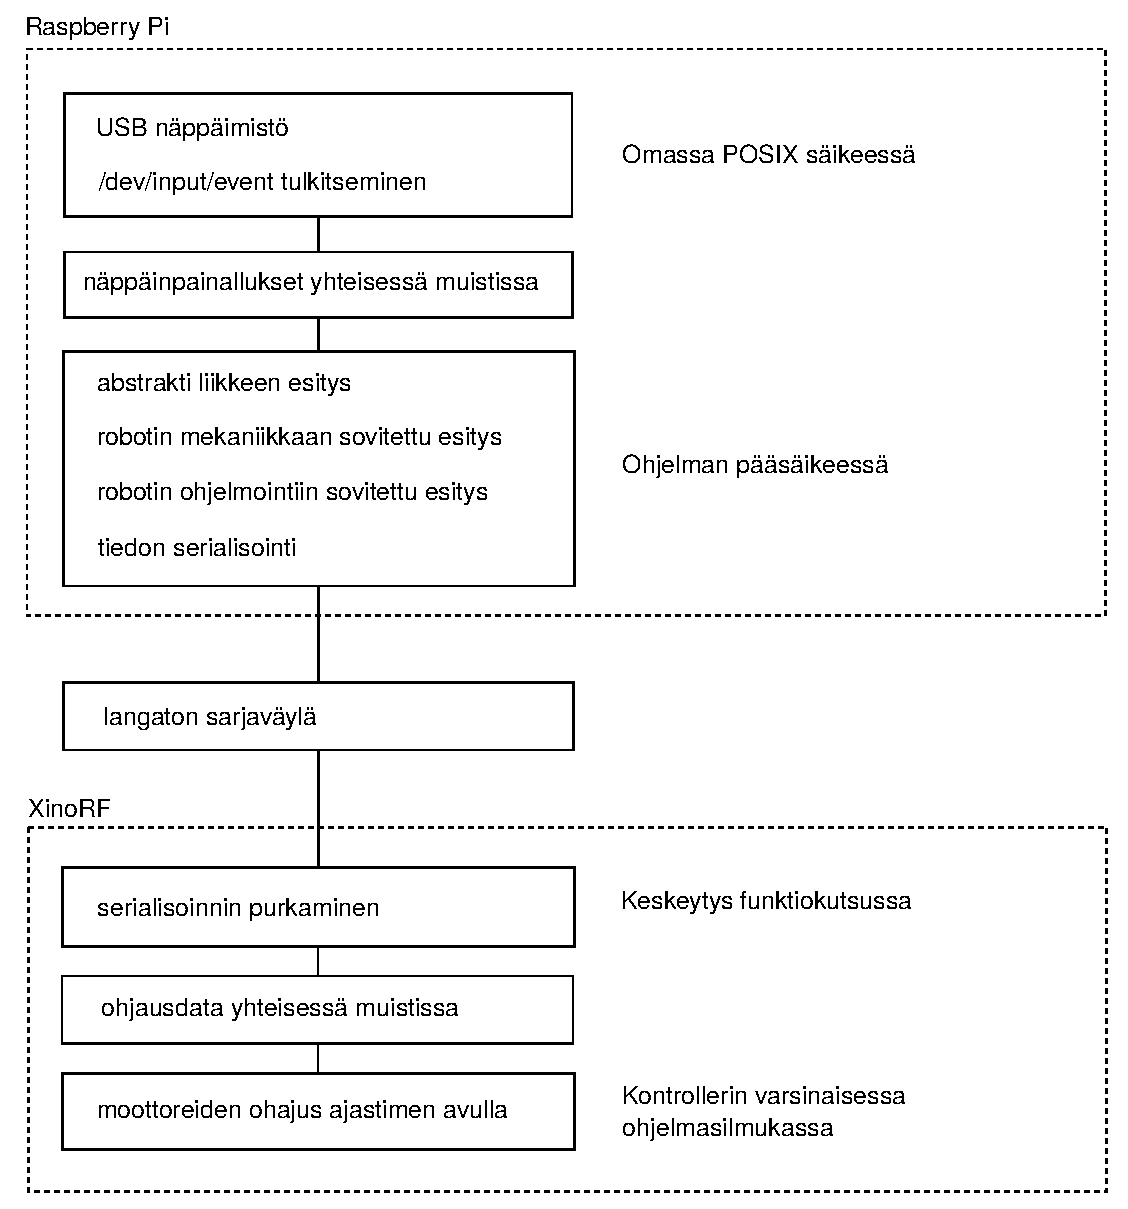
\includegraphics[scale=0.5]{./architechture.pdf}
\end{figure}

\subsection{Käyttöliittymä}
\label{sec:Kayttoliittyma}

Käyttöliittymä robotin ojausta varten toteutettiin RaspberryPi -alustalla.
Robotin ohjaus käyttöliittymän kautta tapahtuu kokonaan RPI:n liitetyn ulkoisen USB näppäimistön kautta.

\subsubsection{USB käyttöliittymälaitteiden tulkitseminen}
\label{sub:USB kayttoliittymalaitteiden tulkitseminen}

Näppäimistön kautta annetut käskyt luetaan erityisestä \verb+/dev/input/eventX+ tiedostosta. Näppäinpainalluksia tulkitseva moduuli on toteutettu tiedostossa \verb+src/hid_input.c+.

Näppämistöä tulkistseva koodia suoritetaan omassa ohjelma säikeessään. Säikeen aloittaminen on toteutettu käyttämällä POSIX säikeitä.

Uuden säikeen aloittavalle \verb+pthread_create()+ funktiolle annetaan kolmanneksi argumentiksi funktio-osoitin funktioon joka halutaan suorittaa uudessa säikeessä. Neljäntenä argumenttina annetaan yksi \verb+void *+ muutuja jonka kautta kaikki funktion argumentit annetaan. Tässä toteutuksessa argumenttina on pelkkä \verb+void *+:ksi muutettu merkkijonon osoitin \verb+(void *) char *+. Merkkijono kertoo mistä \verb+/dev/input/+ tiedostosta USB näppämimistöä tulkitaan.

\begin{verbatim}
    pthread_t polling_thread_id;
    pthread_create(&polling_thread_id, NULL, hid_polling_loop, (void *)hid_device);
\end{verbatim}

Ohjelman säikeiden välillä siiretään dataa yhteisessä muistissa olevan muuttujan kautta. Yksi säkeistä aina muokkaa dataa ja toinen aina lukee, joten ei tarvittu toteuttaa mutex-järjestelmään tiedon eheyden varmistamiseksi.


 

\subsection{Kineettinen malli}
\label{sub:Kineettinen malli}

Robotin toteuttamista varten sovellettiin useaa eri mateemaattista mallinnusta robotin oletetusta käyttäytymisestä.
Mallit phojautuvat hyvin tunnettuihun ohjausmalleihin joiden oikea toimivuus on näyhty käytännön sovelluksissa jo ennestään.

Mekaanisesti robotti on rakennettu niin, että liikkuminen toteutetaan kahdella laitteen sivuilla sijaitsevan renkaan avulla.
Robotti liikkuu käyttäen kahta ns. differentiaalista ajo-moottoria.
Käytännössä tämä tarkoittaa sitä, että sivulla olevia moottoerita voidaan ohjeta toisitaan riippumatta.
Robotti kääntyy kun renkaat pyörivät eri nopeutta suhteessa toisiinsa.

Robotin ohjaamista varten käytetty matemaattinen malli on seuraavanlainen:
\begin{align}
    \label{equ:diff-drive-implementation}
    \begin{dcases}
        \dot x = \cfrac{R}{2} (v_r + v_l) \cos (\phi)\\
        \dot y = \cfrac{R}{2} (v_r + v_l) \sin (\phi)\\
        \dot \phi = \cfrac{R}{L} (v_r - v_l)   
    \end{dcases}
\end{align}

Robotin oletetaan kulkevan tasaisen tason pinnalla. $x$ ja $y$ kuvaavat laitteen paikkaa tasolla, $\phi$ robotin etuosan osittamaa suuntaan, $v_r$ ja $v_l$ ovat oikean sekä vasemmanpuolisen renkaan pyörimisnopeudet. Lisäksi mallissa esiintyy vakio $R$ joka on ohjaukseen käytettyjen renkaiden säde. Vakio $L$ on renkaiden etäisyys toisistaan.



Yllä esitelty malli toimii hyvin ohjausta varten.
Ohjausalgorimejä kehittäessä päädyttiin kuitenkin siihen tulokseen, että järjestelmää kannattaa käsitellä  yksinkertaisemalla mallilla. Robotin liikkeitä on hankala hahmottaa ajattelemalla pelkästään renkaiden pyörimisnopeutta.

Ohjausalgoritmien kehittämistä varten käytetty matemaattinen malli on seuraavanlainen:
\begin{align}
    \label{equ:diff-drive-design}
    \begin{dcases}
        \dot x = v \cos(\phi)\\
        \dot y = v \sin(\phi)\\
        \dot \phi = \omega
    \end{dcases}
\end{align}

Mallin avulla voidaan määrittää robotin liikke käyttäen hyväksi pelkästään sen translaatio nopeutta $v$ sekä kulmanopeutta $\omega$.

Soveltamalla malleja (\ref{equ:diff-drive-implementation}) ja (\ref{equ:diff-drive-design}) saadaan robotin translaation sekä rotaation ($v$ ja $\omega$) ja renkaiden pyörimisnopeuksien ($v_r$ ja $v_l$) välille korrelaatio joka on helppo toteutta C-kielellä:
\begin{align}
    \label{equ:diff-drive-correlation}
    &
    \begin{dcases}
        v &= \cfrac{R}{2} (v_r + v_l)\\
        \omega &= \cfrac{R}{L} (v_r - v_l)\\
    \end{dcases}
    &
    \begin{dcases}
        v_r &= \cfrac{2v + \omega L}{2R}\\
        v_l &= \cfrac{2v - \omega L}{2R}\\
    \end{dcases}
\end{align}


Muunnos on toteutettu tiedostossa \verb+src/dynamical_model.c+


\subsection{Kommunikointi protokolla}
\label{sec:Kommunikointi protokilla}

Sarjaväylän kommunikaatio toteutettiin AVRllä käyttäen mikro-ohjaimen tuottamaa ISR -funktiokutsua joka tapahtuu aina kun sarjavälälle on saapunut tavu dataa. \verb+printf()+ ja \verb+scanf()+ -perheen funktioiden vaatimat \verb+stdout+ ja \verb+stdin+ puskurit toteutettiin myös, mutta funktioita ei kuitenkaan päädytty käyttämään suuren ROM vaatimuksien takia (yli 1000 tavua pelkän \verb+printf()+ käyttämistä varten).

Robotti tallentaa viimeksi saadut komennot muistiin, joten uusi komentoja tarvitsee lähettää sarjaväylän yli vain sillon kun niihin on tapahtunut muutos. Näin vältytään toistuvilta samanlaisilta viesteiltä.

\subsubsection{Viestin rakenne}
\label{sub:Viestin rakenne}


Vestit ovat kiinteän mittaisia, ja sisältävät aina samat kentät. Viesti voidaan esitää C-kiellä seuraavanlaisella tietorakenteella:


\begin{verbatim}
    struct command_message {
        uint16_t id;
        uint16_t tick_period_right;
        uint16_t tick_period_left;
        char direction;
        char checksum;
    } __attribute__((packed));
\end{verbatim}

\begin{center}
\begin{tabular}{|r|c|c|c|c|c|c|}
    \hline
    Nimi & \verb+start+ & \verb+id+ & \verb+right_tick_period+ & \verb+left_tick_period+ & \verb+direction+ & \verb+checksum+ \\
    \hline
    Koko & 8 bit & 16 bit & 16 bit & 16 bit & 8 bit & 8 bit\\
    \hline
\end{tabular}
\end{center}


\paragraph{start:} kiinteästi määritelty bittikuvio \verb+0x61+ joka vastaa ascii merkkiä \verb+'a'+. Merkin tarkoitus on välttää sitä, että vastaanottaja yrittää tulkita kaikkea sarjaväylään saapuvaa dataa. Johtuen siitä, että data tulee radion kautta, `turhaa' dataa joka on tarkoitettu jonkin muun laitteen vastaanotettavaksi saapuu melko paljon. Viestiä ei ruveta purkamaan ennen kuin merkki on vastaanotettu.

Yllä \verb+start+ tavu on tietoisesti jätetty pois structista koska se ei sisällä uutta dataa

\paragraph{id:} 16 bitin pituinen laitekohtainen tunnistuskoodi. Koodin tehtävänä on mahdollistaa usean samanlaisen robotin ohjaamisen samalla alueella, ilman että järjestelmien viestiliikenteet häiritsevät toisiaan. Koodi on tarkoitus tallentaa robotin pitkäaikaiseen EEPROM muitsiin jotta se säilyy vaikka laite sammutetaan (toistaiseksi toiminto on viellä toteuttamatta).

\paragraph{right- sekä left\_tick\_period:} kertoo kuinka monen ajatimen aikayksikön välein robotin askelmoottoriden tulee ottaa askel. Tarkemmin kohdassa \ref{sec:Moottorien ohjaaminen}.
 
\paragraph{direction:} 8 bitin pituinen bittijono, josta alimmat kaksi bittiä on käytössä. Alin bitti määrää oikean puolen moottorin pyörimis-suunnan ja toisiksi alin bitti määrää vasemman moottorin suunnan.

\paragraph{checksum:} Tiiviste arvo jonka avulla voidaan havaita väärin formatoitu data. Tiiviste saadaan laskemalla \verb+id+, \verb+tick_period_right+, \verb+tick_period_left+ sekä \verb+direction+ kentätä muodastavien tavujen XOR tulo. 


\subsection{Moottorien ohjaaminen:}
\label{sec:Moottorien ohjaaminen}

\begin{figure}
    \centering
    \caption{Askelmoottoreita ohjaava tilakone}
    \label{fig:stepper_fsm}
    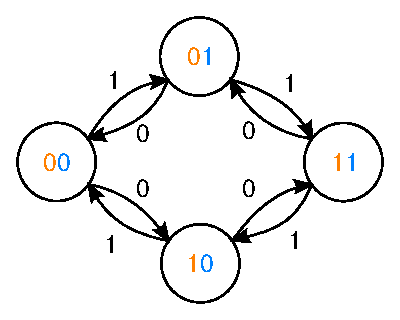
\includegraphics[scale=0.8]{./stepper_fsm.pdf}
\end{figure}
\begin{figure}
    \centering
    \caption{Tilakoneen lähtö ajan funktiona kun tulossa (suunta) on 1}
    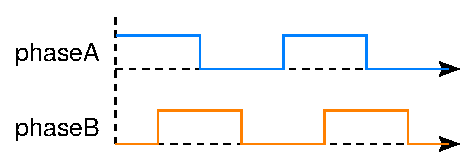
\includegraphics[scale=0.8]{./stepper_timing.pdf}
\end{figure}



Moottorieden ohjausta varten käytetään 16-bittistä ajastinta. Ajastimen esijakaja on asetttu olemaan 1024 ja mikro-ohjaimen kellotaajuus on 16 MHz. Tästä saadaan kello jonka tarkkuus (yhden aikayksikön pituus) on $1024/16 \text{ MHz} = 64 \mu s $. Ajastimen laskin kierähtää takaisin nollaan $2^{16} * 64\mu s \approx 4.2 s$ välein. 

Funktiota \verb+stepper_tick()+ kutsutaan aina kun sopiva määrä aikaa on kulunut. Funkito on toteutettu yksinkertaisella tilakoneella (Kuva \ref{fig:stepper_fsm}).

Funktion täysi prototyyppin on \verb+stepper_tick(struct *stepper_state_machine, char direction)+. Ensimmäinen argumentti on osoittaja tietorakenteeseen joka määrittelee moottorin jolla halutaan ottaa askel. Toinen argumentti määrittää suunnan johon askel otetaan (tilakoneen tulo).

Moottorin määrittelevään tietorakenteeseen on tallenettu I/O -nastat joihin tilakoneen lähtö on kytketty sekä kyseistä moottoria ohjaavan tilakoneen tila:

\begin{verbatim}
    struct stepper_state_machine {
        uint8_t phaseA_pin;
        uint8_t phaseB_pin;
        volatile uint8_t *phaseA_port;
        volatile uint8_t *phaseB_port;
        char state;
    };
\end{verbatim}

Tietorakenteen \verb+state+ kentän arvot on valittu niin, että alin ja toisiksi alin bitti määrittävät \verb+phaseA+ sekä \verb+phaseB+ nastojen tilan.

\section{Oppitulosket}
\label{sec:Oppitulosket}


Suuri osa työskently- ja oppimisprosessia koostui eri asiaankuuluvien C otsaketiedostojen lukemisesta, koska tietoa ei suurikaan muualta löytynyt helposti. 
Esimerkiksi USB käyttöliitymälaitteiden raa'an datan tulkistemista varten ei löytynyt kovin perusteellista oppimateriaalia verkosta.

\subsection{Rekisteriosoittimien käsittely}
\label{Rekisteriosoittimien kasittely}

Yksi kiinnostava asia oli keskiä millä datatyypillä AVR:n erikoistoimintorekisterit (SFR) niin kuin \verb+PORTB+ ovat esitetty.
Esitytavan tunteminen oli olennaista jotta pystyi kirjoittamaan tehokkaita funktioita joille annetaan I/O -nasta argumenttina. Arduino/wiring kirjastoja käyttäessä kuluu paljon laskutehoa siihen, että siirrytään Arduinon nastojen numeroinnista AVR yhteensopivaan esitystapaan. Käsittelemällä rekisterejen osoittajia saadaan huomattavasti nopeammin suoritettavaa koodia.

Esitystapaa tuli käytettyä stepperimoottoreiden määrittelyssä.



\subsection{Struct teitorakenteiden esitys muistissa}

\verb+Struct+ tietorakentiden vertaileminen eri arkkitehtuureilla oli myös kiinnostavaa.
RPI:n 32-bittin ARM arkkitehtuuri pyrkii asettamaan datan muistiosotteisiin jotka ovat neljällä jaollisia. 8-bittinen AVR ei kuitenkaan muistiosoitteiden jaollisuudesta välitä.
Tämä johtaa siihen, että structiin pakattua dataa ei voida turvallisesti siirtää suoraan ARM arkkitehtuurilta AVR arkkitehtuurille ilman että erikseen vamistetaan että tietorakenteiden esitys todella on sama molemmilla arkkitehtuuriella.
Kirjoittaessa koodia jota on tarkoitus suorittaa molemilla arkkitehtuureilla pitää pitää mielessä että myös datatyyppien koot eroavat toisistaan. AVR:n \verb+int+ muuttuja on 16-bittinen, kun 32-bittisen ARM:n datatyyppi on 32-bittinen.
Yleispätevää koodia saa kuitenkin kirjoitettua käyttämällä \verb+<inttypes.h>+ määrittämiä datapyyppejä kuten \verb+uint8_t+ ja \verb+int32_t+

\subsection{Puskuroimaton kirjoitus päätteelle}
\label{sub:Puskuroimaton kirjoitus paatteelle}

Virheen korjaus viestejä kannataa tulostaa päätteellä käyttämällä \verb+fprintf(stderr, ...)+ tavallisen \verb+printf()+ sijasta, varsinkin kun työstää aika-kriittistä koodia. Puskuroidun tulostuksen sivuvaikutus tuli esiin, kun RPIllä suoritettava ohjelma käyttäytyi eri tavall riippuen siitä, että suoritettiinko se itsenäisesti vai \verb+strace+ analysoimana. 

  
\subsection{Käytä oikeaa datalehteä}
\label{sub:Kayta oikeaa datalehtea}


Ojelmoitaessa PWM lähtöä (ei käytössä lopullisessa järjestlmässä) moottoreiden ohjaamista varten oli vahingossa ATmega8 datalehti käytössä ATmega328 datalehden sijaan. Mikrokontrollert ovat melkein samanlaiset, mutta niissä ei kuitenkaan ole identtiset ajastimet, eikä koodi toiminut. 


\end{document}
